\chapter{Testing}

When the classifier is trained, testing can begin. This is done in the testing window, as shown below. All of the trained gestures should now be visible along the Y-axis of the plot.\\

\begin{figure}[H]
    \centering
    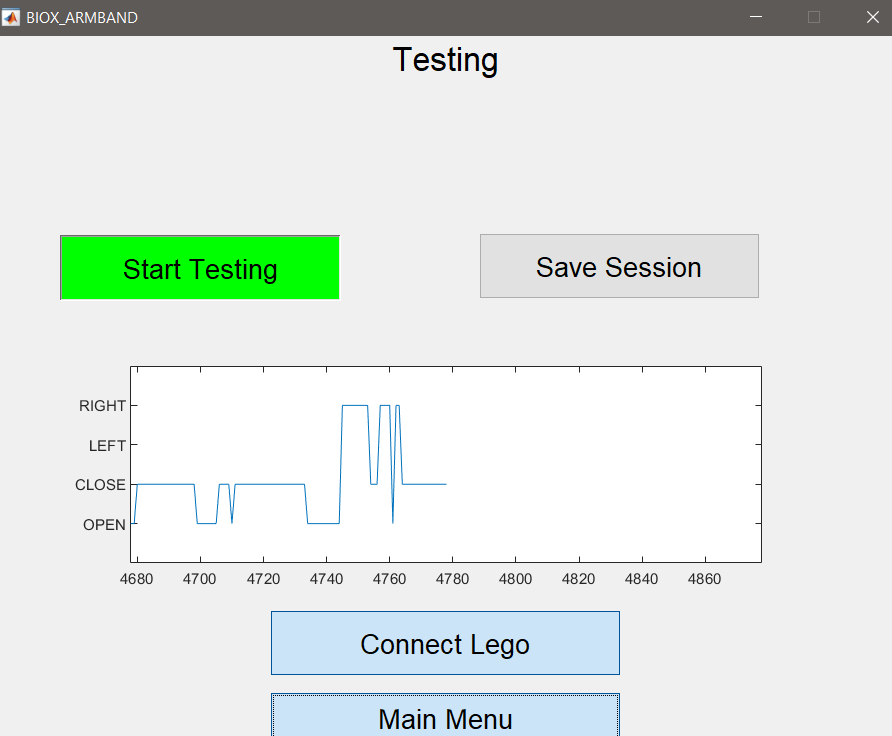
\includegraphics[width=0.6\linewidth]{figures/AppPics/5_TESTING2.PNG}
    \caption{Testing menu.}
    \label{fig:my_label}
\end{figure}

\begin{enumerate}[label=\textbf{Step \arabic*}:]
    \item Start by clicking the \textbf{"Start Testing"} button. This will turn green, indicating that the test is running.
    \item Perform the trained gestures one at the time, to confirm that the training is done correctly.
    \item If everything is in order, a connection with LEGO Mindstorm can be made. Make sure bluetooth is re-enabled and click the \textbf{"Connect Lego"} button. The connection can take some time, and should end with the LEGO Mindstorm device starting to move.
    \item The LEGO Mindstorm device should now be able to follow directions based on the performed gestures.
    \item To end testing, click the \textbf{"Stop Testing"} button to finish.
    \item All collected data can be exported to excel by clicking the \textbf{"Save Session"} button.
    \item When the data is saved successfully, Main Menu will appear automatically.
\end{enumerate}
